\documentclass[a4paper,11pt,notitlepage]{article}
\usepackage{amsmath}
\usepackage{amsfonts}
\usepackage{amssymb}
\usepackage[UTF8]{ctex}
\usepackage{graphicx}
\usepackage{color}
\usepackage{changepage}
\usepackage{enumitem}
\usepackage{subfigure}
\usepackage{float}
\usepackage[backend=biber]{biblatex}

\usepackage{titlesec}
\titleformat{\section}{\bfseries\Large}{$\S$\,\thesection}{1em}{}
\titleformat{\subsection}{\bfseries\large}{\Roman{subsection}}{1em}{}
\titleformat{\subsubsection}{\bfseries\normalsize}{\roman{subsubsection}}{1em}{}
\titlespacing*{\subsection}{2em}{2pt}{2pt}
\titlespacing*{\subsubsection}{3em}{2pt}{2pt}
\title{\vspace{-1.5cm} \textbf{\huge{数值分析第5章上机}}\vspace{-1em}}
\author{By 211870125 陈睿硕}
\date{}

\usepackage{geometry}
\geometry{left=2cm,right=2cm,top=2cm,bottom=2cm}

\usepackage{fancyhdr}
\pagestyle{fancy}
\fancyhf{}
\fancyhead[L]{Chapter 5}
\fancyhead[R]{\thepage}
\setlength{\headheight}{14pt}

\usepackage{listings}  % 引入 listings 包
\lstset{                % 定义代码块的样式
    basicstyle=\normalsize\ttfamily, % 设定代码字体大小、样式
    showspaces=false,   % 不显示空格
    showstringspaces=false, % 不显示字符串中的空格
    showtabs=false,     % 不显示制表符
    frame=single,       % 设定代码块边框样式
    rulecolor=\color{black}, % 设定代码块边框颜色
    tabsize=4,          % 设定制表符长度为 4 个字符
    captionpos=t,       % 设定标题位置为底部
    keywordstyle=\bfseries\color{blue}\ttfamily,
    stringstyle=\color{red}\ttfamily,
    commentstyle=\color{green}\ttfamily,
    morecomment=[l][\color{magenta}]{\#},
    framesep=0.5em,
    frameround=tttt,
    breaklines=true,    % 自动换行
    breakatwhitespace=false, % 只在空格分割处换行
    escapeinside={\%*}{*)}   % 允许使用 LaTeX 命令
}
\renewcommand{\lstlistingname}{代码}

\usepackage{hyperref}
\usepackage{cleveref}
\crefname{theorem}{定理}{定理}
\crefname{figure}{图}{图}
\crefname{equation}{式}{式}
\crefname{listing}{代码}{代码}

\begin{document}
\maketitle
\vspace{-1cm}
\thispagestyle{fancy}

\section{问题}
\begin{adjustwidth}{1em}{0pt}
\begin{enumerate}[label=\textbf{Q\arabic*}]
    \item 数学上已经证明$\int^{1}_{0}f(x)dx=\pi$,其中$f(x)=\frac{4}{1+x^2}$。分别使用复合梯形,复合 Simpson 求积公式计算
          $\pi$的近似值。选择不同的 h , 对每种求积公式,试将误差刻画成对每种求积公式,试将误差刻画成 h 的函数,
          并比较两方法的精度。是否存在某个 h 值,当低于这个值之后再继续减小 h 的值,计算不再有所改进?为什么?\label{Q1}\notag
    \item 实现 Romberg 求积方法,重复\ref{Q1}的过程。\label{Q2}\notag
    \item 实现 自适应积分方法,重复\ref{Q1}的过程。\label{Q3}\notag
    \item 用所掌握的所有数值积分方法计算积分$\int_{0}^{\infty}\frac{x^3}{e^x-1}dx$,
          并比较不同方法的计算效率和精度。\label{Q4}\notag
\end{enumerate}
\end{adjustwidth}

\section{算法思路}
\subsection{对\ref{Q1}的解答}
我们实现了复合梯形,复合 Simpson 求积方法,代码见\cref{code1.1}。得到h和误差(绝对值)的关系如\cref{pic:1}。
\begin{figure}[H]
    \centering
    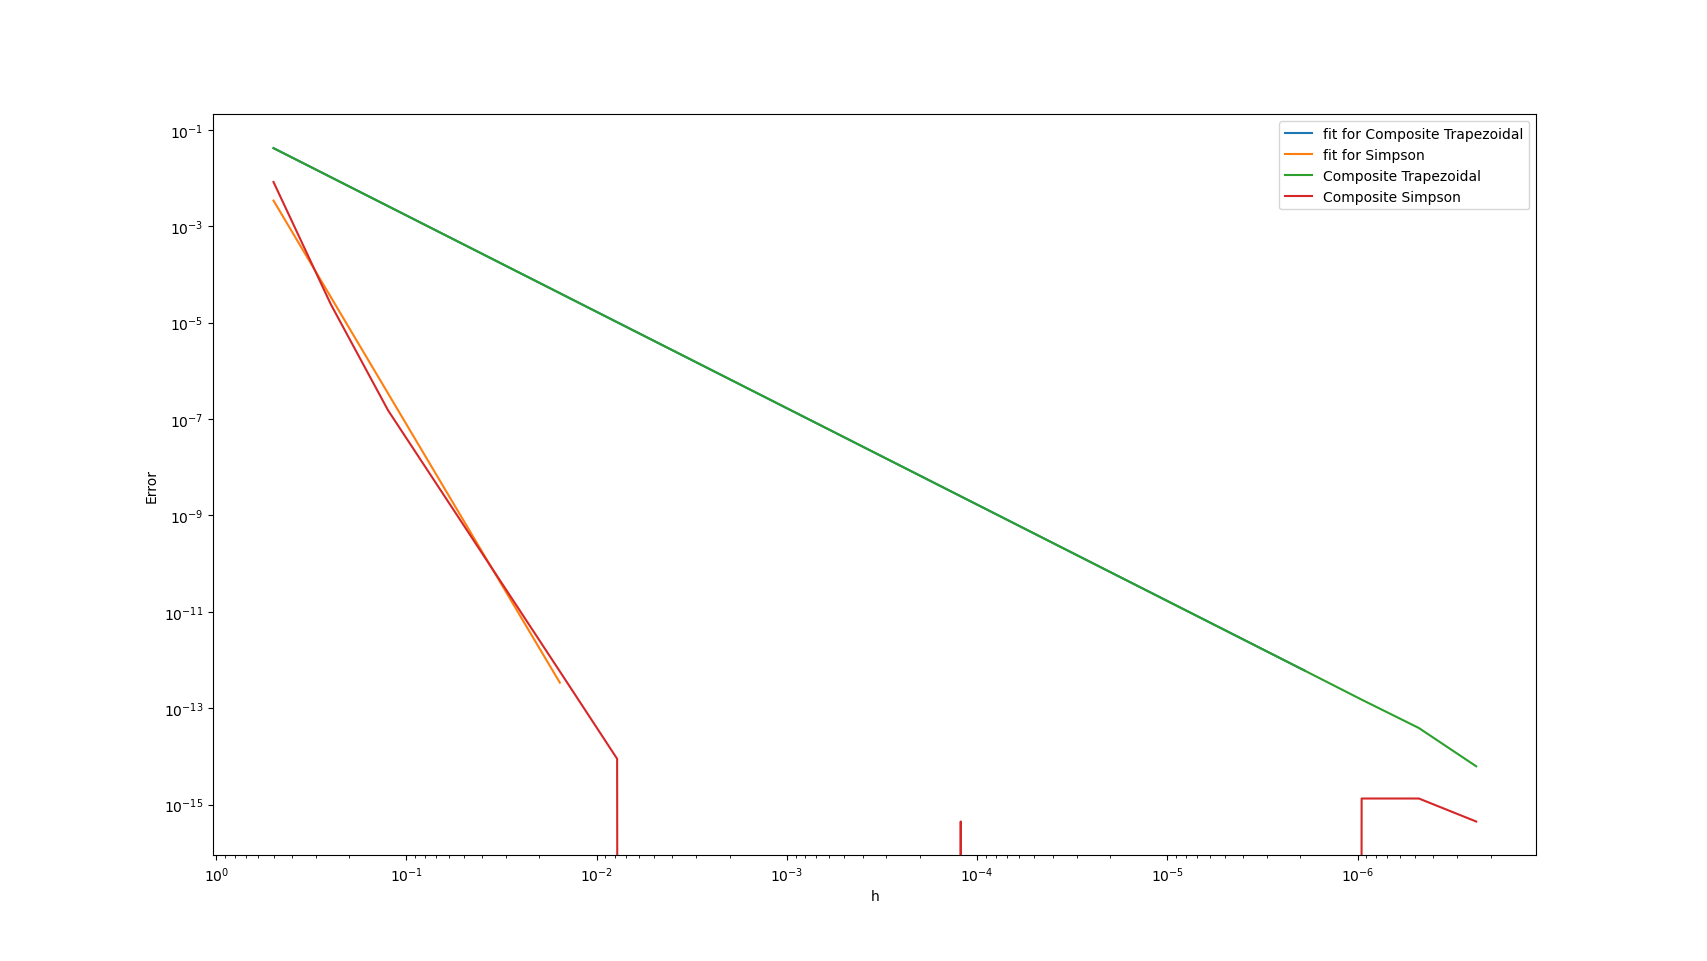
\includegraphics[width=0.8\textwidth]{../picture/Fifth_Chapter_1A.png}
    \caption{复合梯形,复合 Simpson 求积法的误差随h的变化}
    \label{pic:1}
\end{figure}

\subsection{对\ref{Q2}的解答}
使用Python实现,代码见\cref{code1.2}。得到h和误差(绝对值)的关系如\cref{pic:2}。
\begin{figure}[H]
    \centering
    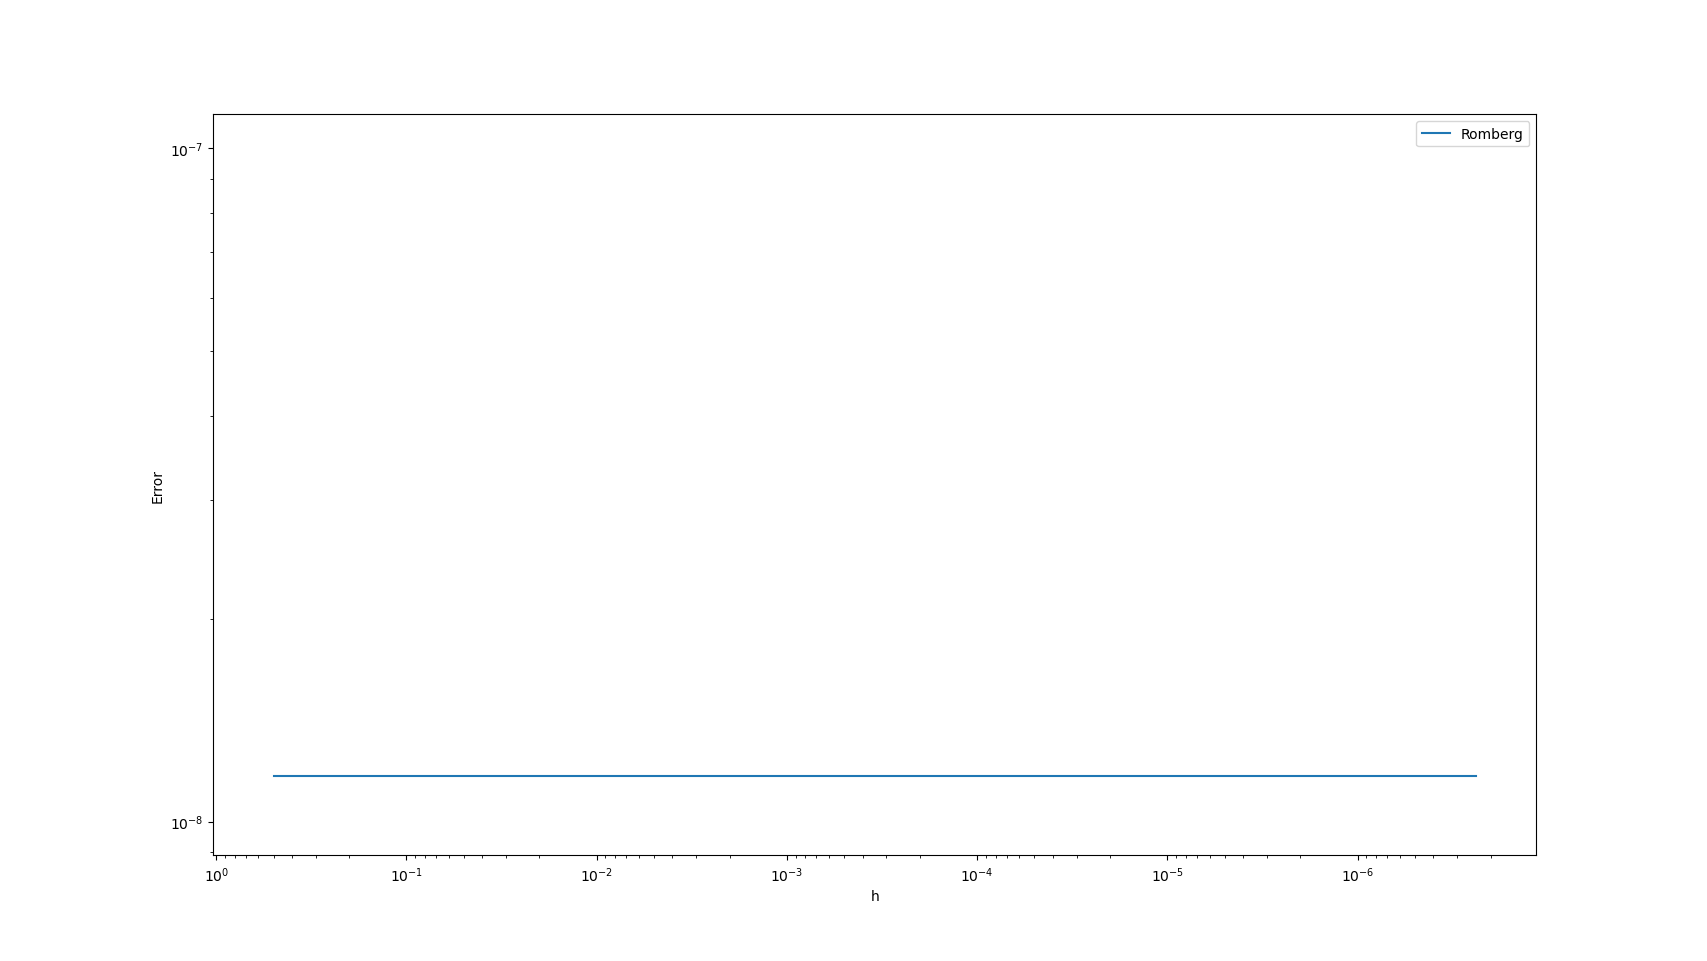
\includegraphics[width=0.8\textwidth]{../picture/Fifth_Chapter_1B.png}
    \caption{Romberg求积法的误差随h的变化}
    \label{pic:2}
\end{figure}

\subsection{对\ref{Q3}的解答}
使用Python实现,代码见\cref{code1.3}。得到h和误差(绝对值)的关系如\cref{pic:3}。
\begin{figure}[H]
    \centering
    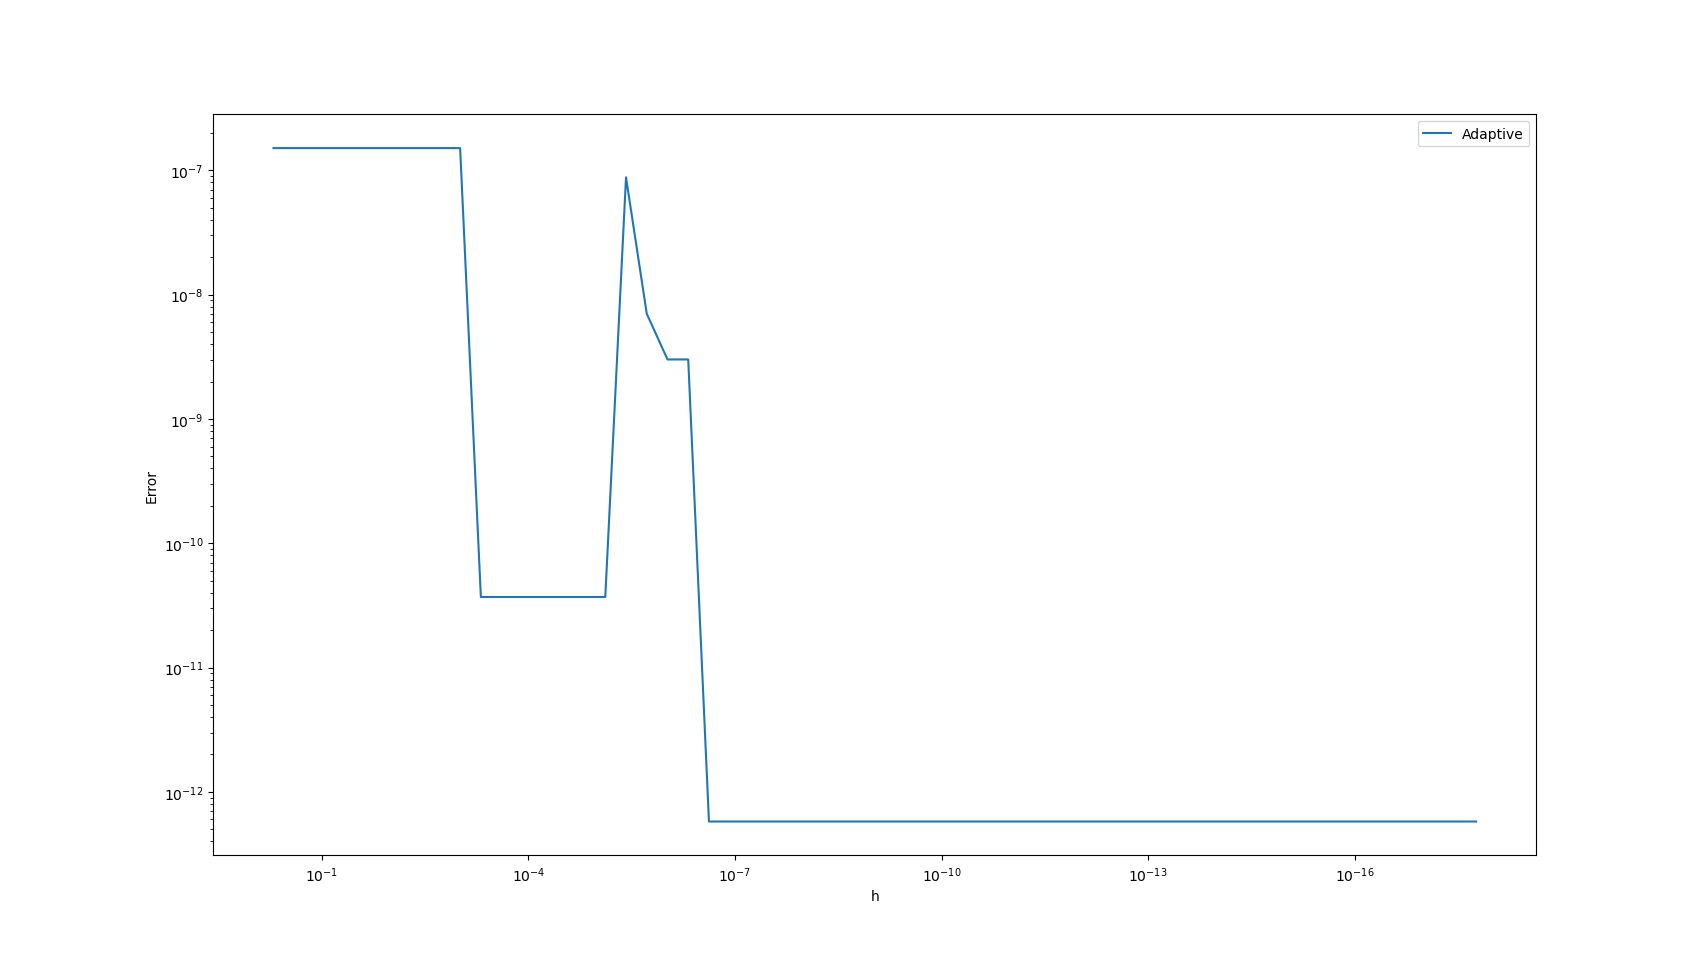
\includegraphics[width=0.8\textwidth]{../picture/Fifth_Chapter_1C.png}
    \caption{自适应Simpson积分方法的误差随h的变化}
    \label{pic:3}
\end{figure}

\subsection{对\ref{Q4}的解答}
首先,我们使用$t=\frac{1}{1+x}$的坐标变换将积分区间从$[0,+\infty]$变换到$[0,1]$,并补充定义0和1处的函数值为0。
然后我们使用了复合梯形公式、复合Simpson公式、Romberg积分法、自适应积分法计算变换后的积分,代码见\cref{code2.1}。
得到计算出的误差(用数学方法可以算出此积分的精确值为$\frac{\pi^4}{15}$)和h的关系如\cref{pic:4}。
\begin{figure}[H]
    \centering
    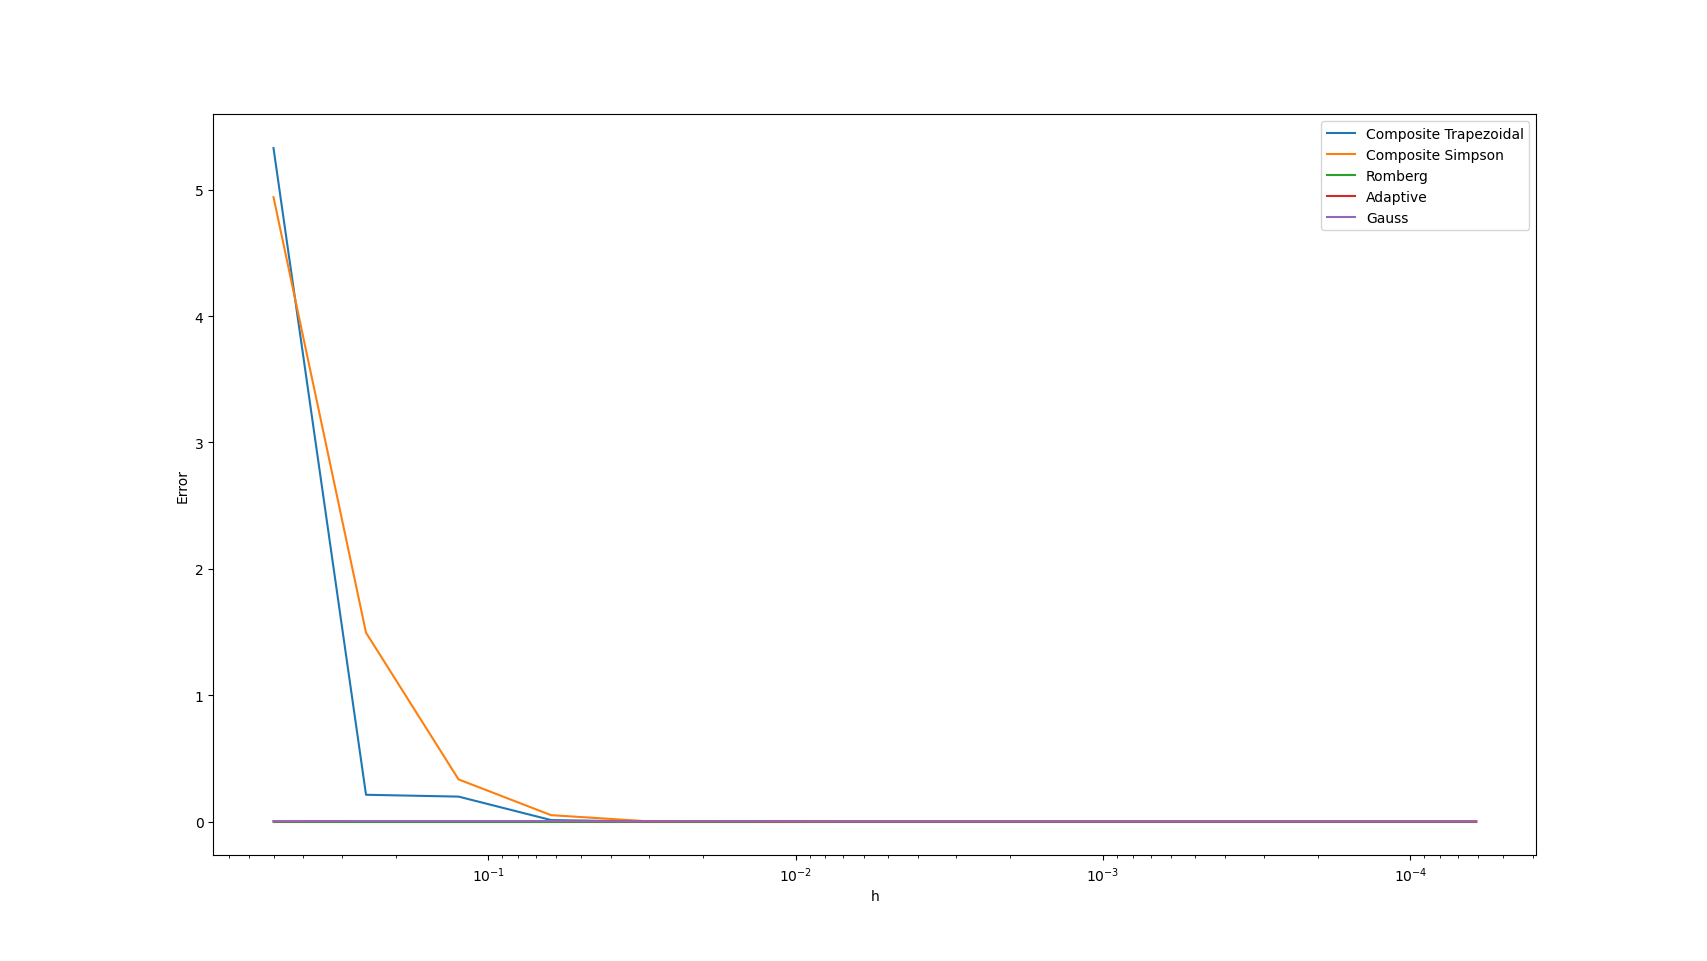
\includegraphics[width=0.8\textwidth]{../picture/Fifth_Chapter_2.png}
    \caption{多种方法计算积分的误差}
    \label{pic:4}
\end{figure}
得到各种方法在h取不同值的计算时间如\cref{pic:5}。
\begin{figure}[H]
    \centering
    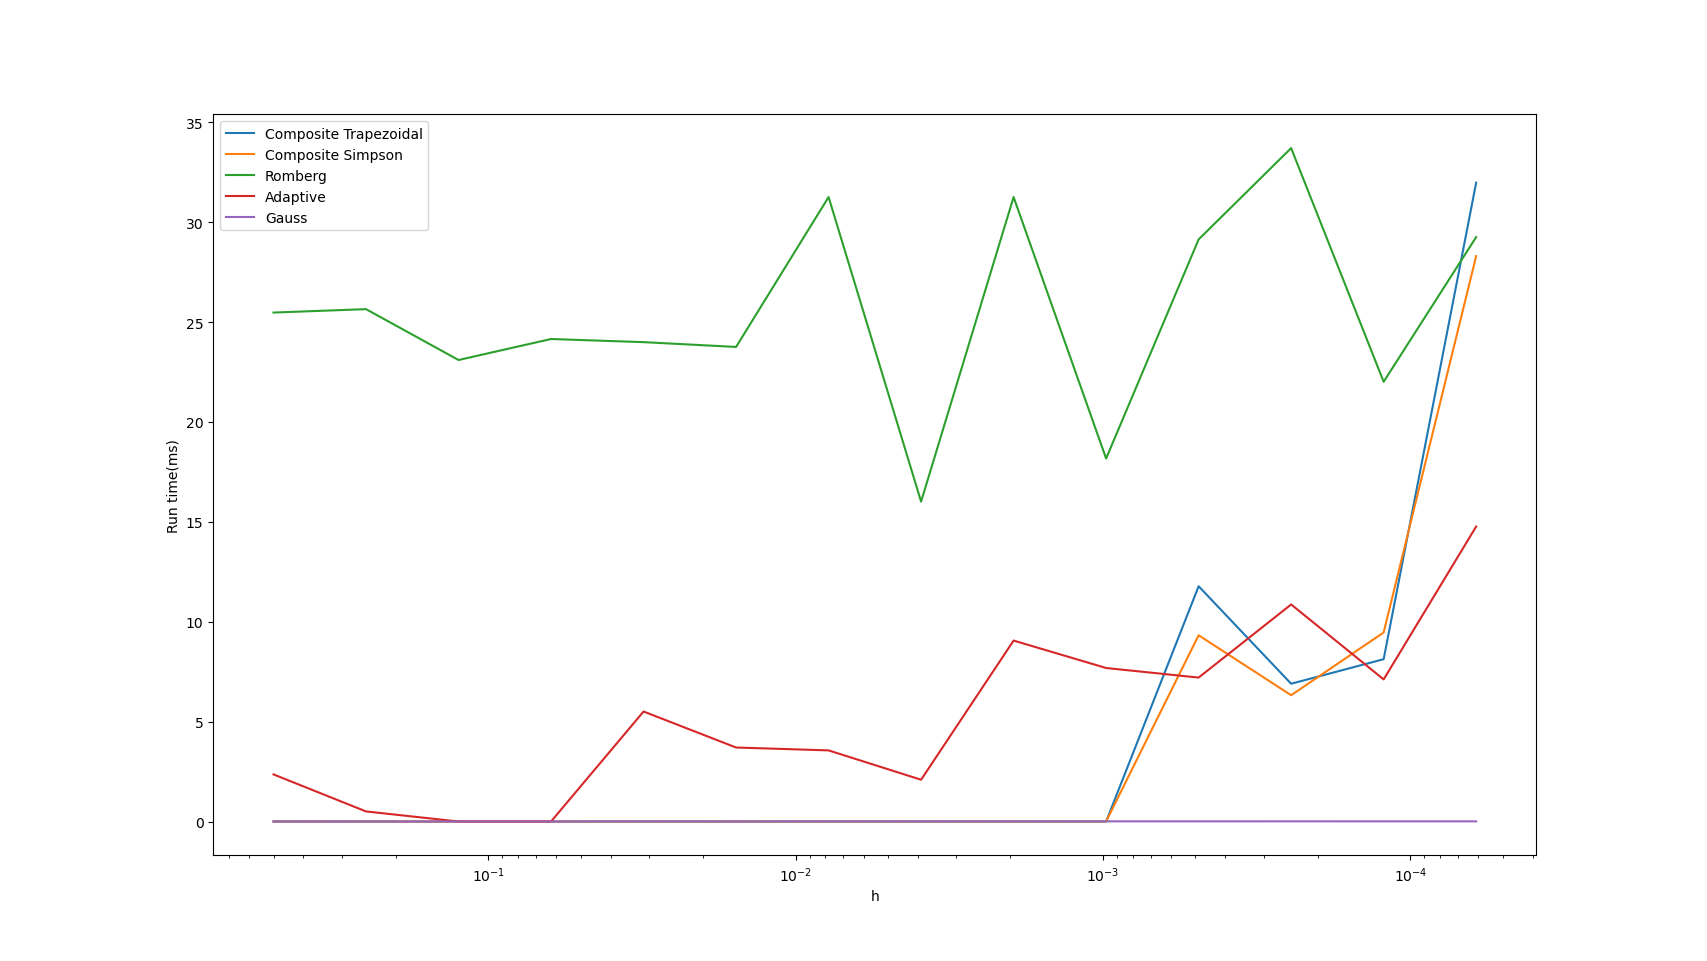
\includegraphics[width=0.8\textwidth]{../picture/Fifth_Chapter_2(1).png}
    \caption{多种方法计算积分的运行时间}
    \label{pic:5}
\end{figure}

\section{结果分析}
\subsection{对\ref{Q1}的分析}
可以看到,h和误差的关系在h不特别小时几乎是对数线性关系,对于复合积分法$Error\approx 10^{-0.77821}h^{2.0000}$,
而对于复合Simpson法$Error\approx 10^{-0.46800}h^{6.6460}$。\\
\indent 我们知道,复合梯形公式的误差(绝对值)$Error=\frac{1}{12}h^2f''(\xi )$,其中$\xi \in (0,1)$,
这与我们的估计式相吻合($f''(x)$在$[0,1]$上变化不大)。\\
\indent 而复合Simpson公式的误差(绝对值)$Error=\frac{1}{180}h^4f''(\xi )$,其中$\xi \in (0,1)$,
这就与我们的估计式有一定的差距,可能是因为函数拟合的位置h值还比较大,也可能是这个被积函数所特有的“过收敛现象”。\\
\indent h小于$10^{-2}$次时,复合Simpson求积法的误差不再发生明显缩小,因为此时舍入误差对误差的贡献开始提升。

\subsection{对\ref{Q2}的分析}
我们可以看到,随着h的减小,误差几乎没有变化,这是因为在Romberg积分法迭代时,每迭代一次,插值点间的距离便会缩小一半,
所以算法的效果并不很依赖于初始的h值。

\subsection{对\ref{Q3}的分析}
我们可以看到,误差变动很大,但在h小于$10^{-7}$后稳定在了一个值,这应该是因为每一个小区间中积分的误差都已经小于规定的阈值($10^{-6}$)。

\subsection{对\ref{Q4}的分析}
各种方法的最小、最大误差和对于某个h计算使用的最长时间如下:
\begin{center}
\begin{tabular}{|c|c|c|c|}
\hline
Method & Min error & Max error & Run time(ms) \\
\hline
复合梯形 & 8.881784197001252e-16 & 5.3299859885281755 & 31.97479248046875\\
\hline
复合Simpson & 8.881784197001252e-16 & 4.942001517281957 & 28.298377990722\\
\hline
Romberg & 8.881784197001252e-15 & 8.881784197001252e-15 & 33.70404243469238\\
\hline
自适应Simpson & 1.8865497430908817e-07 & 0.0036696045968218627 & 14.763355255126953\\
\hline
复合Gauss两点 & 1.8865497430908817e-07 & 0.0036696045968218627 & 8.5732936859\\
\hline
\end{tabular}
\end{center}
\textbf{注:Romberg求积法中不同的迭代终止条件会极大地影响算法的结果与运行时间,
于是我们设置了最大迭代次数为14作为唯一的终止条件,使其运行时间与其他方法较为接近,以便比较。}\\
\indent 结合上表、\cref{pic:4}和\cref{pic:5},复合梯形公式与复合Simpson公式在h足够小时误差能够达到浮点数下界,
但运行时间较长,并且需要随着h的减小收敛;Romberg求积法得益于多次的迭代,对初始的h值非常不敏感,运行时间长但能够始终维持
误差几乎不变。而自适应和复合Gauss两点求积法能达到的精度较低,但运行时间有较大优势,同时误差始终保持在一个较低水准,稳定性很强。\\
\indent 不过事实上,我们可以发现,h在$10^{-3}$次处复合梯形公式和复合Simpson公式的运行时间几乎为0,但是此处计算的误差已经
达到$10^{-15}$的量级,所以从单个任务的应用来说,我们可以选取合适的h,使用复合梯形或者复合Simpson求积法达到时间和精度的完美平衡。

\section{附录:程序代码}
\begin{lstlisting}[language=Python,caption={Fifth Chapter 1A.py},label={code1.1}]
import numpy as np
import matplotlib.pyplot as plt


def f(x):
    return 4 / (1 + x**2)


def composite_trapezoidal(a, b, h):
    n = int((b - a) / (2 * h)) * 2
    x = np.linspace(a, b, n+1)
    y = f(x)
    s = (y[0] + y[n] + 2 * np.sum(y[1:n])) * h / 2
    return s


def composite_simpson(a, b, h):
    n = int((b - a) / h)
    x = np.linspace(a, b, n+1)
    y = f(x)
    s = (y[0] + y[n] + 4 * np.sum(y[1:n:2]) + 2 * np.sum(y[2:n-1:2])) * h / 3
    return s


a, b = 0, 1

trap_errors = np.array([])
simp_errors = np.array([])

h_values = np.array([0.5**i for i in range(1, 23)])

for i in h_values:
    trap_error = np.abs(composite_trapezoidal(a, b, i) - np.pi)
    simp_error = np.abs(composite_simpson(a, b, i) - np.pi)
    trap_errors = np.append(trap_errors, trap_error)
    simp_errors = np.append(simp_errors, simp_error)

mask1 = np.where(h_values > 1e-6)
coefficients1 = np.polyfit(
    np.log10(h_values[mask1]), np.log10(trap_errors[mask1]), 1)
# 输出拟合的函数式
print(
    f"对于复合梯形公式拟合的函数式为 log10(y) = {coefficients1[0]}log10(x) + {coefficients1[1]}")

mask2 = np.where(h_values >= 10**(-2.1))
coefficients2 = np.polyfit(
    np.log10(h_values[mask2]), np.log10(simp_errors[mask2]), 1)
# 输出拟合的函数式
print(
    f"对于复合梯形公式拟合的函数式为 log10(y) = {coefficients2[0]}log10(x) + {coefficients2[1]}")

poly_fit1 = np.poly1d(coefficients1)
poly_fit2 = np.poly1d(coefficients2)
plt.plot(h_values[mask1], np.power(10, poly_fit1(
    np.log10(h_values[mask1]))), label='fit for Composite Trapezoidal')
plt.plot(h_values[mask2], np.power(10, poly_fit2(
    np.log10(h_values[mask2]))), label='fit for Simpson')
plt.plot(h_values, trap_errors, label="Composite Trapezoidal")
plt.plot(h_values, simp_errors, label="Composite Simpson")
plt.xscale('log')
plt.yscale('log')
plt.xlabel('h')
plt.ylabel('Error')
plt.gca().invert_xaxis()
plt.legend()
plt.show()    
\end{lstlisting}

\begin{lstlisting}[language=Python,caption={Fifth Chapter 1B.py},label={code1.2}]
import numpy as np
import matplotlib.pyplot as plt


def f(x):
    return 4 / (1 + x**2)

def romberg(f, a, b, h, max_iterations=20, epsilon=1e-7):
    R = [[0] * (max_iterations + 1) for _ in range(max_iterations + 1)]
    R[0][0] = 0.5 * (b - a) * (f(a) + f(b))
    for i in range(1, max_iterations + 1):
        h = (b - a) / (2 ** i)
        sum = 0.0
        for k in range(1, 2 ** (i - 1) + 1):
            x = a + (k - 0.5) * 2 * h
            sum += f(x)
        R[i][0] = 0.5 * R[i - 1][0] + h * sum
        for j in range(1, i + 1):
            R[i][j] = (4 ** j * R[i][j - 1] - R[i - 1][j - 1]) / (4 ** j - 1)
            if j==i and np.abs(R[i][j]-R[i][j-1])<epsilon:
                return R[i][j]
    return R[max_iterations][max_iterations]

a, b = 0, 1

romberg_errors = np.array([])

h_values = np.array([0.4**i for i in range(1, 15)])

for i in h_values:
    romberg_error = np.abs(romberg(f, a, b, i) - np.pi)
    romberg_errors = np.append(romberg_errors, romberg_error)

plt.plot(h_values, romberg_errors, label="Romberg")
plt.xscale('log')
plt.yscale('log')
plt.xlabel('h')
plt.ylabel('Error')
plt.gca().invert_xaxis()
plt.legend()
plt.show()
\end{lstlisting}

\begin{lstlisting}[language=Python,caption={Fifth Chapter 1C.py},,label={code1.3}]
import numpy as np
import matplotlib.pyplot as plt


def f(x):
    return 4 / (1 + x**2)

def composite_simpson(f, a, b, h):
    n = int((b - a) / (2 * h)) * 2
    x = np.linspace(a, b, n+1)
    y = f(x)
    s = (y[0] + y[n] + 4 * np.sum(y[1:n:2]) + 2 * np.sum(y[2:n-1:2])) * h / 3
    return s

def adaptive_integration(f, a, b, h, epsilon=1e-6, max_depth=50):
    x0 = a
    x2 = b
    x1 = (a + b) / 2.0
    S0 = composite_simpson(f, a, b, (b-a)/2)
    S1 = composite_simpson(f, x0, x1, (x1-x0)/2)
    S2 = composite_simpson(f, x1, x2, (x2-x1)/2)
    error = abs(S0 - S1 - S2)
    if error < epsilon or max_depth == 0:
        return S1 + S2
    else:
        left_integral = adaptive_integration(
            f, x0, x1, epsilon / 2, h / 2, max_depth - 1)
        right_integral = adaptive_integration(
            f, x1, x2, epsilon / 2, h / 2, max_depth - 1)
        return left_integral + right_integral


a, b = 0, 1

adaptive_errors = np.array([])

h_values = np.array([0.5**i for i in range(1, 60)])

for i in h_values:
    adaptive_error = np.abs(adaptive_integration(f, a, b, i) - np.pi)
    adaptive_errors = np.append(adaptive_errors, adaptive_error)

plt.plot(h_values, adaptive_errors, label="Adaptive")
plt.xscale('log')
plt.yscale('log')
plt.xlabel('h')
plt.ylabel('Error')
plt.gca().invert_xaxis()
plt.legend()
plt.show()    
\end{lstlisting}

\begin{lstlisting}[language=Python,caption={Fifth Chapter 2.py},label={code2.1}]
import matplotlib.pyplot as plt
import time

def f(t):
        return t**3 / (1 - t)**5 * 1/(np.exp(t / (1 - t))-1) if t!=0 and t!=1 else 0


def composite_trapezoidal(f, a, b, h):
    n = int((b - a) / (2 * h)) * 2
    x = np.linspace(a, b, n+1)
    y = list(map(f, x))
    s = (y[0] + y[n] + 2 * np.sum(y[1:n])) * h / 2
    return s


def composite_simp_errorson(f, a, b, h):
    n = int((b - a) / h)
    x = np.linspace(a, b, n+1)
    y = list(map(f,x))
    s = (y[0] + y[n] + 4 * np.sum(y[1:n:2]) + 2 * np.sum(y[2:n-1:2])) * h / 3
    return s


def romberg_integration(f, a, b, h, max_iterations=14, epsilon=1e-13):
    R = [[0] * (max_iterations + 1) for _ in range(max_iterations + 1)]
    R[0][0] = 0.5 * (b - a) * (f(a) + f(b))
    for i in range(1, max_iterations + 1):
        h = (b - a) / (2 ** i)
        sum = 0.0
        for k in range(1, 2 ** (i - 1) + 1):
            x = a + (k - 0.5) * 2 * h
            sum += f(x)
        R[i][0] = 0.5 * R[i - 1][0] + h * sum
        for j in range(1, i + 1):
            R[i][j] = (4 ** j * R[i][j - 1] - R[i - 1][j - 1]) / (4 ** j - 1)
    return R[max_iterations][max_iterations]


def adaptive_integration(f, a, b, h, epsilon=1e-6, max_depth=50):
    x0 = a
    x2 = b
    x1 = (a + b) / 2.0
    S0 = composite_simp_errorson(f, a, b, (b-a)/2)
    S1 = composite_simp_errorson(f, x0, x1, (x1-x0)/2)
    S2 = composite_simp_errorson(f, x1, x2, (x2-x1)/2)
    error = abs(S0 - S1 - S2)
    if error < epsilon or max_depth == 0:
        return S1 + S2
    else:
        left_integral = adaptive_integration(
            f, x0, x1, epsilon / 2, h / 2, max_depth - 1)
        right_integral = adaptive_integration(
            f, x1, x2, epsilon / 2, h / 2, max_depth - 1)
        return left_integral + right_integral


def composite_gauss_twopoint(f, a, b, h):
    x = np.array([-np.sqrt(1/3), np.sqrt(1/3)])
    w = np.array([1, 1])
    n = (b - a) / h
    intervals = np.linspace(a, b, n+1)
    integral = 0
    for i in range(n):
        x_new = (x + 1) * intervals[i] / 2 + (1 - x) * intervals[i+1] / 2
        integral += h/2 * np.sum(w * f(x_new))
    return integral

a, b = 0, 1
h_values = np.array([0.5**i for i in range(1, 15)])

trap_errors = np.array([])
trap_times=np.array([])
for i in h_values:
    _st = time.time()
    trap = np.abs(composite_trapezoidal(f, a, b, i))
    _ed=time.time()
    trap_errors = np.append(trap_errors, np.abs(trap-np.power(np.pi,4)/15))
    trap_times=np.append(trap_times,_ed-_st)
print(f"复合梯形公式最小误差:{np.min(trap_errors)},最大误差:{np.max(trap_errors)},最多用时(ms):{1000*max(trap_times)}")

simp_errors = np.array([])
simp_times=np.array([])
for i in h_values:
    _st = time.time()
    simp = np.abs(composite_simp_errorson(f, a, b, i))
    _ed = time.time()
    simp_errors = np.append(simp_errors, np.abs(simp-np.power(np.pi,4)/15))
    simp_times=np.append(simp_times,_ed-_st)
print(f"复合Simpson公式最小误差:{np.min(simp_errors)},最大误差:{np.max(simp_errors)},最多用时(ms):{1000*max(simp_times)}")

romberg_errors = np.array([])
romberg_times=np.array([])
for i in h_values:
    _st = time.time()
    romberg = np.abs(romberg_integration(f, a, b, i))
    _ed = time.time()
    romberg_errors = np.append(romberg_errors, np.abs(romberg-np.power(np.pi,4)/15))
    romberg_times=np.append(romberg_times,_ed-_st)
print(f"Romberg最小误差:{np.min(romberg_errors)},最大误差:{np.max(romberg_errors)},最多用时(ms):{1000*max(romberg_times)}")

adaptive_errors = np.array([])
adaptive_times=np.array([])
for i in h_values:
    _st = time.time()
    adaptive = np.abs(adaptive_integration(f, a, b, i))
    _ed = time.time()
    adaptive_errors = np.append(adaptive_errors, np.abs(adaptive-np.power(np.pi,4)/15))
    adaptive_times=np.append(adaptive_times,_ed-_st)
print(f"自适应最小误差:{np.min(adaptive_errors)},最大误差:{np.max(adaptive_errors)},最多用时(ms):{1000*max(adaptive_times)}")

gauss_errors=np.array([])
gauss_times=np.array([])
for i in h_values:
    _st = time.time()
    gauss = np.abs(adaptive_integration(f, a, b, i))
    _ed = time.time()
    gauss_errors = np.append(gauss_errors, np.abs(gauss-np.power(np.pi,4)/15))
    gauss_times=np.append(gauss_times,_ed-_st)
print(f"复合Gauss两点最小误差:{np.min(gauss_errors)},最大误差:{np.max(gauss_errors)},最多用时(ms):{1000*max(gauss_times)}")

plt.plot(h_values, trap_errors, label="Composite Trapezoidal")
plt.plot(h_values, simp_errors, label="Composite Simpson")
plt.plot(h_values, romberg_errors, label="Romberg")
plt.plot(h_values, adaptive_errors, label="Adaptive")
plt.plot(h_values, gauss_errors, label="Gauss")
plt.xscale('log')
plt.xlabel('h')
plt.ylabel('Error')
plt.gca().invert_xaxis()
plt.legend()
plt.show()

plt.plot(h_values, trap_times*1000, label="Composite Trapezoidal")
plt.plot(h_values, simp_times*1000, label="Composite Simpson")
plt.plot(h_values, romberg_times*1000, label="Romberg")
plt.plot(h_values, adaptive_times*1000, label="Adaptive")
plt.plot(h_values, gauss_times, label="Gauss")
plt.xscale('log')
plt.xlabel('h')
plt.ylabel('Run time(ms)')
plt.gca().invert_xaxis()
plt.legend()
plt.show()
\end{lstlisting}
\end{document}